%\chapter{det-comp}


%%%%%%%%%%%%%%%%%%%%%%%%%%%%%%%%%%%%%%%%%%%%%%
%\section{Anode Plane Assemblies}

%%%%%%%%%%%%%%%%%%%%%%%%%%%%%%%%%%%%%%%%%%%%%%
\section{Cathode Plane Assemblies}


\subsection{Scope, Requirements and Design Parameters}

The cathode plane is constructed from 6$\times$3 cathode plane assemblies (CPAs) to form the 16m $\times$ 6m area.  It has a HV cup at the beam downstream side to interface with the HV feedthrough. The top and bottom field cage modules are mechanically and electrically connected to the top and bottom edges of the cathode plane.  The cathode plane is suspended through insulating bars to the CPA installation rail.

\subsubsection{Requirements}

\begin{itemize}
\item Provide equipotential surfaces at -180kV nominal bias voltage
\item Maintain a flatness better than 1cm when submerged in the liquid argon
\item Use materials with comparable CTEs to that of stainless steel 
\item Limit the electric field exposed to LAr to under 30kV/cm
\item Prevent damage to the TPC including its readout electronics In case of a HV discharge anywhere on the cathode
\item Provide constant bias voltage and current to all attached field cage resistor divider chains
\item Support the full weight of the 4 connected top/bottom field cage modules and a person on the bottom CPA at installation
\item Accommodate cryostat roof movement between warm and LAr filled states
\item Constructed in modular form that can be easily installed in the cryostat
\item Accommodate PD calibration features
\item Has no trapped volume

\end{itemize}

\subsubsection{Design Parameters}

Width, height, sheet thickness, frame thickness, module width...


\subsection{The need for highly resistive cathode planes}
Stored energy, charge injection to FEE, dominant ionization current density

Summarize key points in DUNE docdb 1320.

\subsection{The Design of the Cathode}

\subsection{Overview}

Introduce the design concept: strong frame with thin resistive cathode surface; field shaping strips cover the frame; HV bus hidden behind the field shaping strips; outer edges of the CPA frame surrounded by the metal profiles used by the field cage.

\begin{cdrfigure}[CPA Concept]{cpa-concept}{The resistive CPA concept. 
 {\bf Left:} A 3d model of a corner of the cathode showing major components {\bf Right:} E field simulation of a portion of the cathode.} 
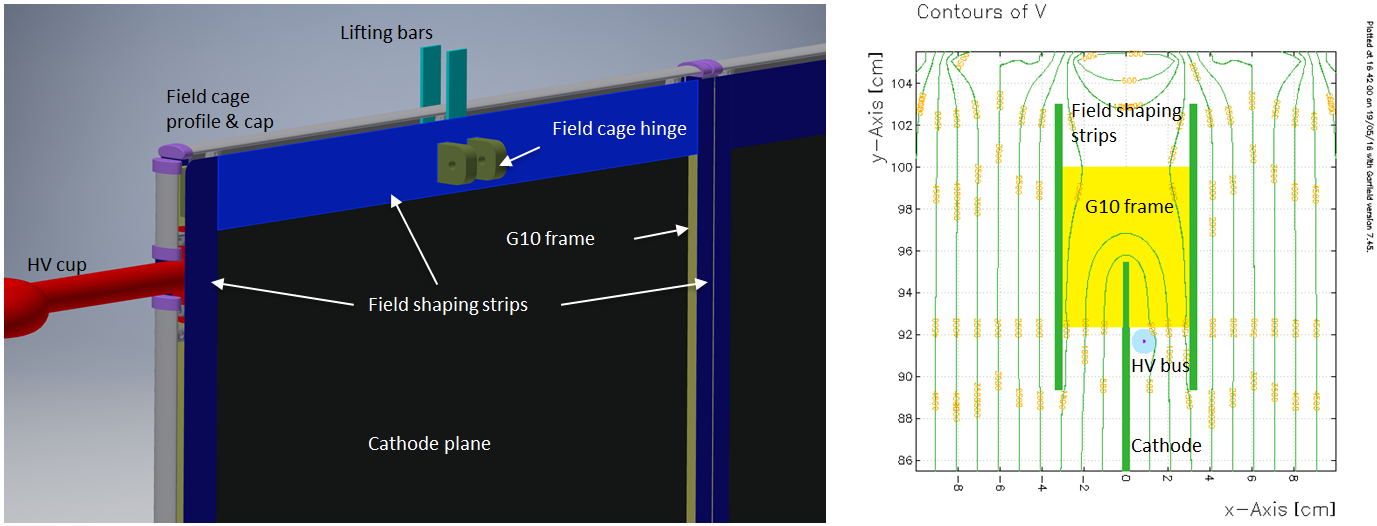
\includegraphics[width=\linewidth]{tpc_cpa_concept.png}
\end{cdrfigure}


\subsubsection{Resistive material}
%% from F. Pietropaolo

The main criteria for the selection of the resistive material to be used for the CPA panels include: 
\begin{itemize}	
\item Surface resistivity range.
\item Compatibility with cryogenic temperatures
\item Robustness to HV discharges, material ageing.
\item Radio-purity.
\item Availability on large area; achievable planarity 
\end{itemize}

Several options have been evaluated.
\begin{itemize}	
\item NORPLEX Micarta NP 315, phenolic laminate loaded with graphite: Intrinsic bulk resistivity in the required range (few M$\Omega$/cm). Density comparable to LAr.
\item Screen printed resistive ink on G10/FR4 substrate (~100 k$\Omega$/square) printed with specific patterns to obtain required average surface resistivity
\item DuPont resistive Kapton film  (25 $\mu$m thickness, graphite loaded, available with resistivity in the 0.5 to 50 M$\Omega$/square range) laminated on G10/FR4 substrate.
\end{itemize}
Also considered at earlier stage:
\begin{itemize}	
\item Zelec ESD powder mixed with polyurethane binder.
\item ESD surface conducting G10 from Current Composite.
\end{itemize}

Radiological tests performed at the LNGS low counting rate facility that G10/FR4 are preferable since MiCarta is more active by orders of magnitude for most relevant radioactive chains.
 
Screen printed ink and Kapton lamination on G10/FR4 are well established fabrication techniques available on panels as large as to 2.1x 1.2 m$^2$ (well matching the CPA panel required size). The screen print technique allows to choose precisely the average surface resistivity value, while Kapton exhibits a more uniform surface and resistivity. 

Tests on large size panels have demonstrated that both options survive without deformation or delamination to repeated immersions in LAr. The resistivity increase at LAr temperature is bounded to less than a factor two for both cases. Electrical contacts are performed with  specific  silver paint paste  highly stable at LAr temperature and resistant to mechanical scratches.

Tests on surface ageing when exposed to HV sparks indicate that Kapton is the preferred solution because:
\begin{itemize}	
\item in the resistive ink case, sparks tend to develop along direction of less resistivity, perpendicular to strip direction inducing a visible degradation of the material surface with some consistent ink evaporation and local measurable change in resistivity (Figure~\ref{fig:cpa-resink}).
\item in the Kapton case instead, sparks are point-like inducing tiny localized carbonization on material surface, at the spark position, but no change in average resistivity is recorded (Figure~\ref{fig:cpa-kapton}). 
\end{itemize}

\begin{cdrfigure}[Resistive ink ageing from sparks]{cpa-resink}{Resistive ink ageing from sparks. 
 {\bf Left:} spark propagation along preferred directions (lower resistivity), {\bf Right:} Status after test: degradation with some material evaporation.} 
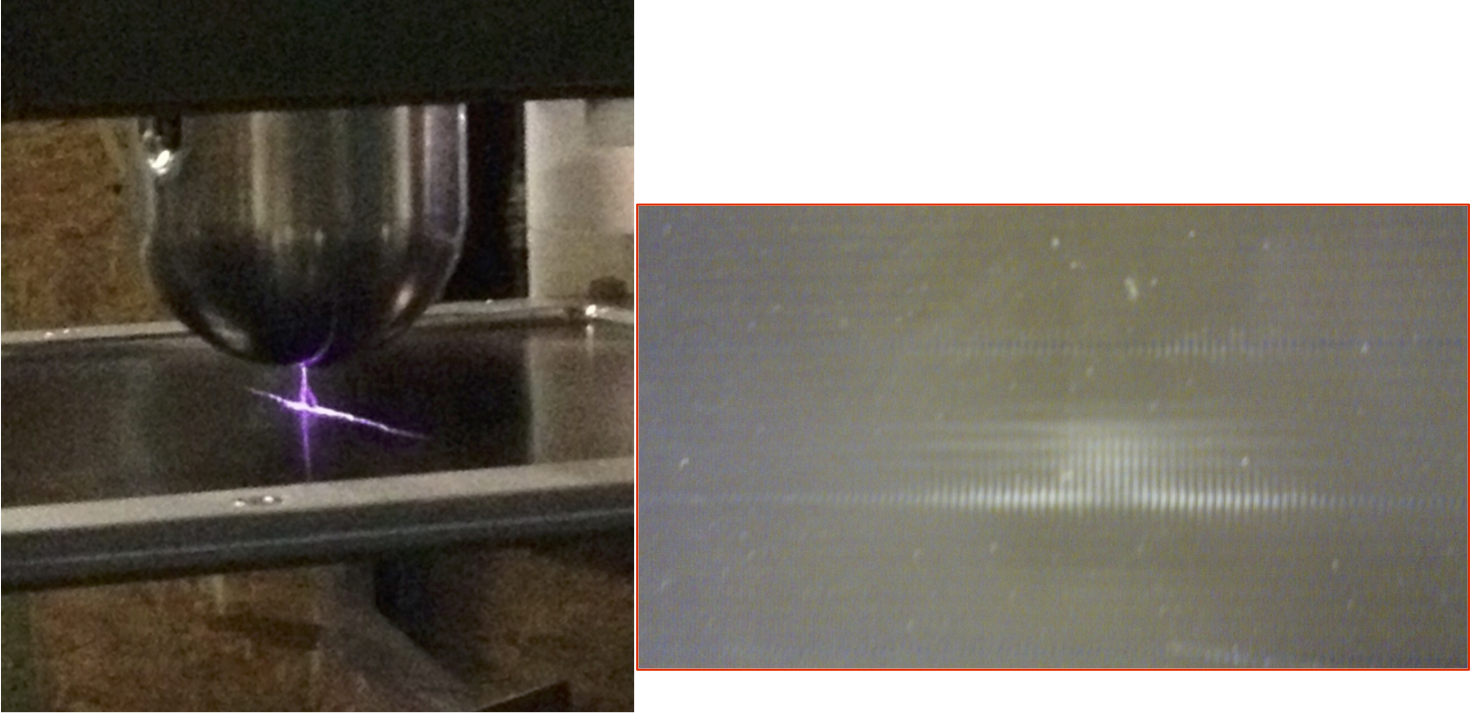
\includegraphics[width=\linewidth]{tpc_cpa-resink.png}
\end{cdrfigure}

\begin{cdrfigure}[The field cage test setup]{cpa-kapton}{Resistive kapton ageing from sparks. 
 {\bf Left:} point-like sparks. {\bf Right:} Localized carbonization on material surface, at the spark position.}
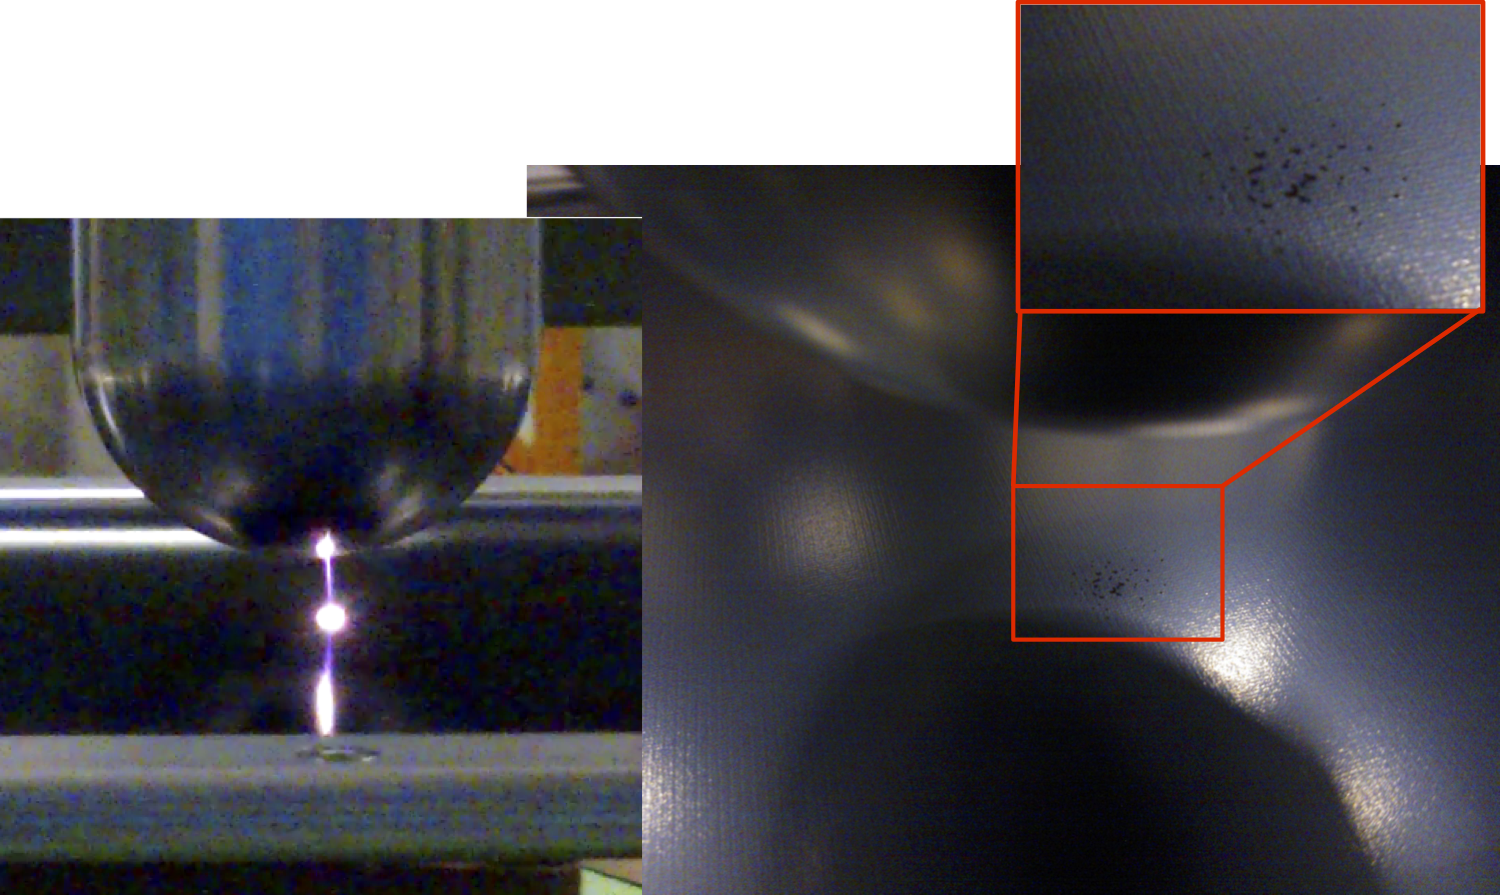
\includegraphics[width=\linewidth]{tpc_cpa-kapton.png}
\end{cdrfigure}

\subsubsection{Support frame material properties}

The main materials for the detector are stainless steel and what is called generically G10 material.  G-10 is a thermosetting industrial fiber glass composite laminate consisting of a continuous filament glass cloth material with an epoxy resin binder. This product, first introduced in the 1950's, has characteristics of high strength, low moisture absorption, excellent electrical properties and chemical resistance. These properties are maintained not only at room temperature but also under humid or moist conditions. NEMA G10 was the designation given to Glass Epoxy sheet composite by the National Electrical Manufacture Association (NEMA) to specify a consistent product between manufactures. 

G10 laminate sheet is made up with difunctional or trifunctional epoxy making up the bulk of heavy sheet and then using finer glass cloth with high temperature resistant tetra-functional epoxy giving a high performance outer finish.

FR4 is the brominated flame retardant version of G 10. The FR 4 material can usually be used where G10 material is specified; however G10 Laminate should not be used where FR-4 is specified.  CERN requires that the material used be flame retardant but halogen free (and therefore bromine free).  FR4 meets the flame retardant requirement but not the halogen free requirement.  Research needs to be conducted into what type of G10/FR4 is available that meets CERN’s requirements.
Another variation of G10 fiberglass sheet is G10 CR laminate used in cryogenic applications. 

Both G-10 and FR-4 are rated at 285 degree F continuous operating temperature. Because they are thermosets, no melting will occur with these grades, however charring will be observed after extended periods above this temperature rating. FR-4 has a UL flammability rating of 94 V-0.

A failure criteria needs to be defined for the G10 material because it is brittle and does not exhibit ductile failure and a defined yield stress like stainless steel.  Brittle materials typically rupture and have a fractional reduction in area due to tensile strain of less than 0.05.  For brittle materials it is recommended that the modified Mohr Theory of Failure be used which states that the principle tensile stresses be less than the ultimate stress of the material.  See Shigley ``Standard Handbook of Machine Design,'' third edition.   Stress concentrations are also a concern for brittle materials and care should be taken to avoid sharp corners and other areas of stress concentrations.  Shigley also defines stress concentration factors which are multipliers for geometric areas where stresses are higher and is a common method for evaluating high stress areas.  

The material properties used for calculations were:

\begin{tabular}{l l}
G10: 	& \\
\hline
Thermal expansion Coefficient	&	$9.6 \times 10^{-6}$ cm/cmK	\\
Modulus of Elasticity			&	2,770ksi				\\
\vspace{0.5em}Ultimate stress				&	32ksi				\\
Stainless Steel: & \\
\hline
Thermal expansion Coefficient	&	$9.6 \times 10^{-6}$ cm/cmK	\\
Modulus of Elasticity			&	30,000ksi				\\
Yield stress					&	36ksi				\\
\end{tabular}


\subsubsection{Mechanical design and stress analysis}
git pu
\begin{cdrfigure}[CPA geometry]{cpa-geometry}{Basic geometry of the CPA array, close ups and a CPA column} 
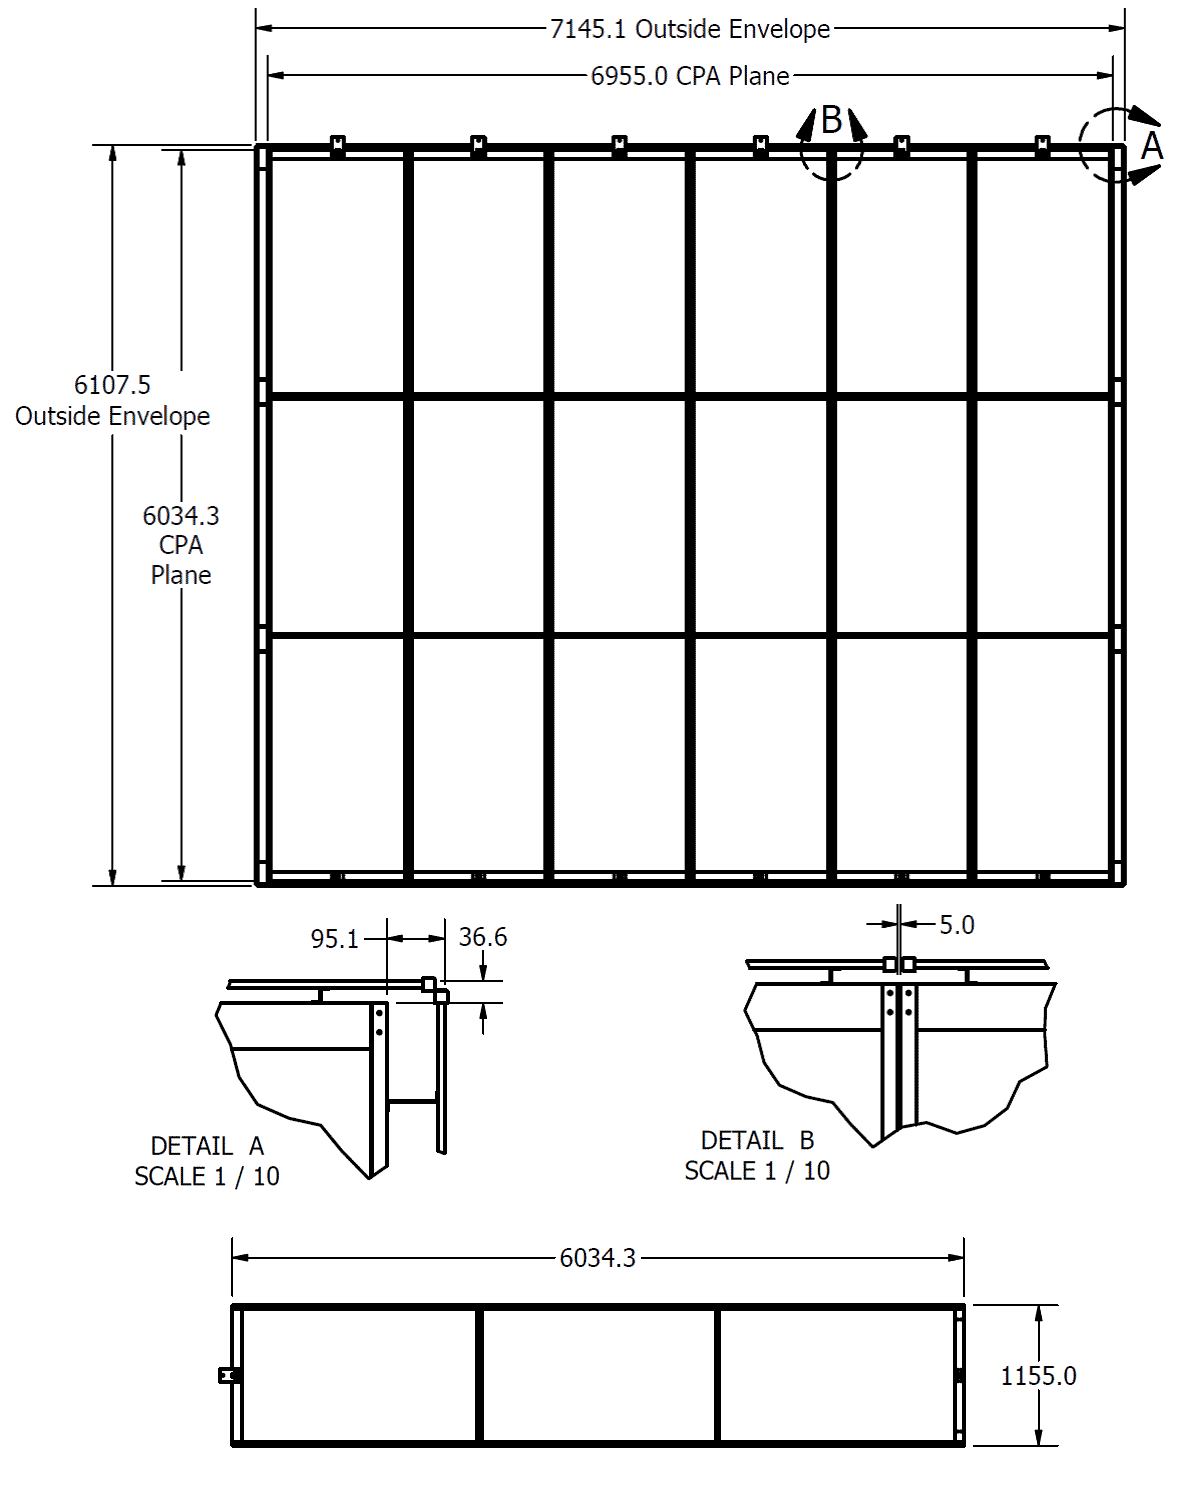
\includegraphics[width=\linewidth]{tpc_cpa_front_views1.png}
\end{cdrfigure}

\begin{cdrfigure}[CPA views2]{cpa-view2}{Views of various part of the CPAs} 
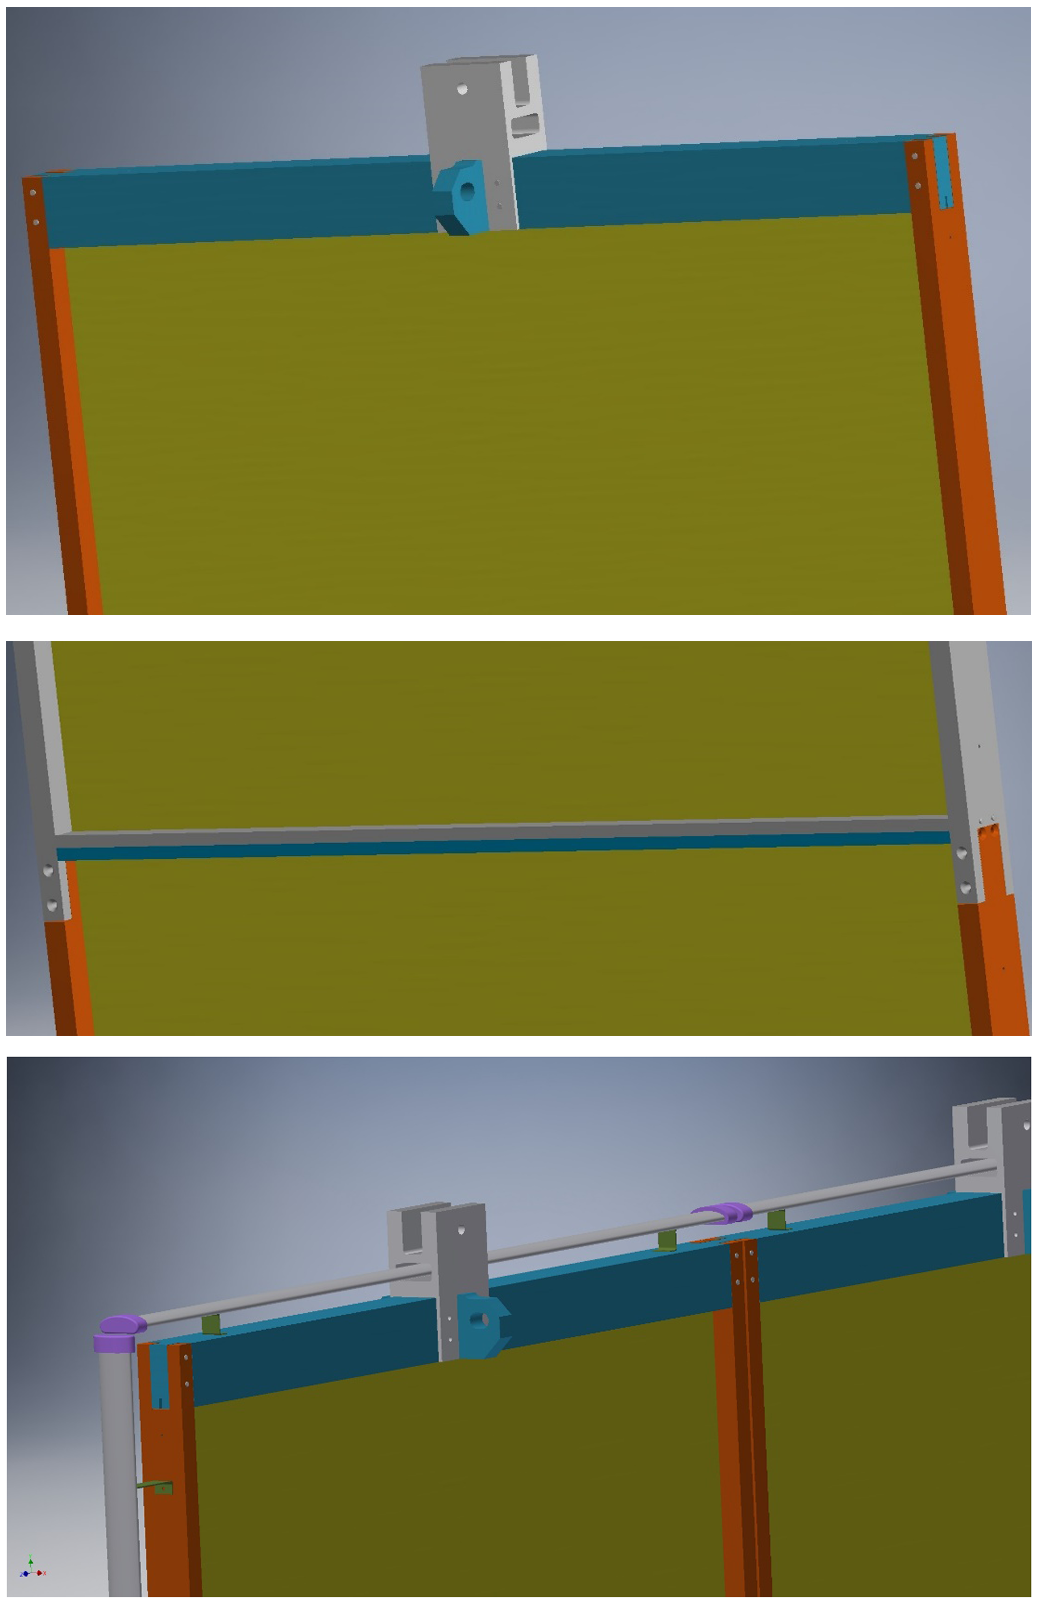
\includegraphics[width=0.8\linewidth]{tpc_cpa_views2.png}
\end{cdrfigure}


Figures~\ref{fig:cpa-geometry} and \ref{fig:cpa-view2} show the basic geometry of the CPA.  The CPA is composed of three modules that are bolted and pinned together with tongue/groove joints to form the full CPA plane.  Each module consists of a framework in which the resistive panel is captured inside a groove.  Each module weights roughly 53 lbs. for a total weight of the CPA plane of 160 lbs.  

The resistive panel is 1/8'' thick G10 and floats within the framework so that no external forces are applied to it.  When hung vertically the weight of the resistive panel (~30lbs per module) rests on the bottom cross bar of the module.  The weight of the modules is transferred through the side bars of the frame and up to the top cross bar, see Figure~\ref{fig:cpa-view2}a.  The very top cross bar of the CPA plane has a block attached to it through which all of the load is transferred to the strap which attaches to the supporting stainless steel I-beam.  

Figure~\ref{fig:cpa-hinge1} shows how the FC will be attached to the assembled CPA plane.  The top and bottom cross bars will have elongated slots through which pins will be inserted to attach the hinged connection.  The weight of the FC is applied to the center of each top and bottom bar.  

\begin{cdrfigure}[CPA and FCA hinged connection]{cpa-hinge1}{The top field cage modules are hung vertically with the CPAs when moved into the cryostat, then rotated to horizontal to attach to the APA} 
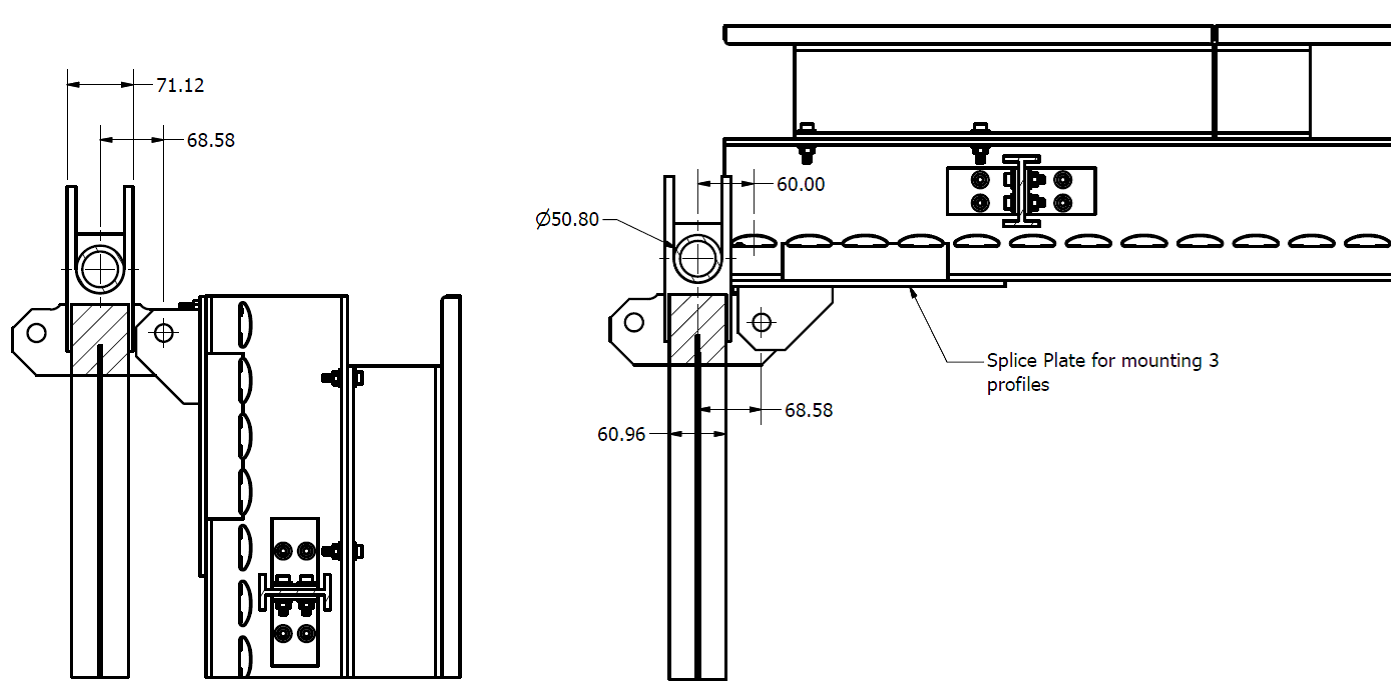
\includegraphics[width=\linewidth]{tpc_cpa_fc_hinge.png}
\end{cdrfigure}


Figure~\ref{fig:cpa-view2}a shows the block at the top of the CPA that is secured to the top cross bar and extends to the top supporting I-beam.  This strap must support the weight of four half FCs (4$\times$220 lbs) and the weight of the CPA itself (160 lbs) for a total weight of 1041 lbs. The section of G10 that connects to the CPA requires and area of only .33 in$^2$ to achieve a safety factor of 10 to the ultimate strength of the G10.  

The strap must have the ability to allow the CPA to pivot and rotate in three directions.  


The CPA frame has been evaluated using empirical and FEA calculations.  The following is a summary of 6 key aspects of the analysis. Detailed calculations are shown in 
\fixme{reference to Vic's writeup}.  

The highest stresses and deflections occur during assembly before the cryostat is filled with liquid.  During installation the CPA must carry the full weight of the FC rather than sharing it with the APA and the buoyancy force which reduces the load from gravity is not present.

In all of the analysis the resistive panels were not included.  In the design of the CPA it is planned that the resistive panel will float within a frame and no load will be applied to it and therefore it does not contribute to the stiffness of the modules.  

{\it A. Lifting the CPA During Installation}

During installation the three frames that make up a CPA module will be placed horizontally on the floor and connected together.  The top of the module will then be secured to the crane and lifted; the bottom of the module will be pivoted on the floor.  By lifting and transversing the hook attached to the top of the module the CPA will be lifted into the vertical position.  The worst case loading occurs immediately after the crane begins to lift the top of the module when it is simply supported at the bottom and top.  The stresses and deflections are small as see in Figure~\ref{fig:cpa-h_load}.   The plane will sag a maximum of roughly 2'' and the stresses are below 2,000psi which is far below the ultimate stress.  

\begin{cdrfigure}[CPA stress in horizontal position]{cpa-h_load}{Stress and deflection of a connected 3 CPA stack in horizontal position supported at both ends} 
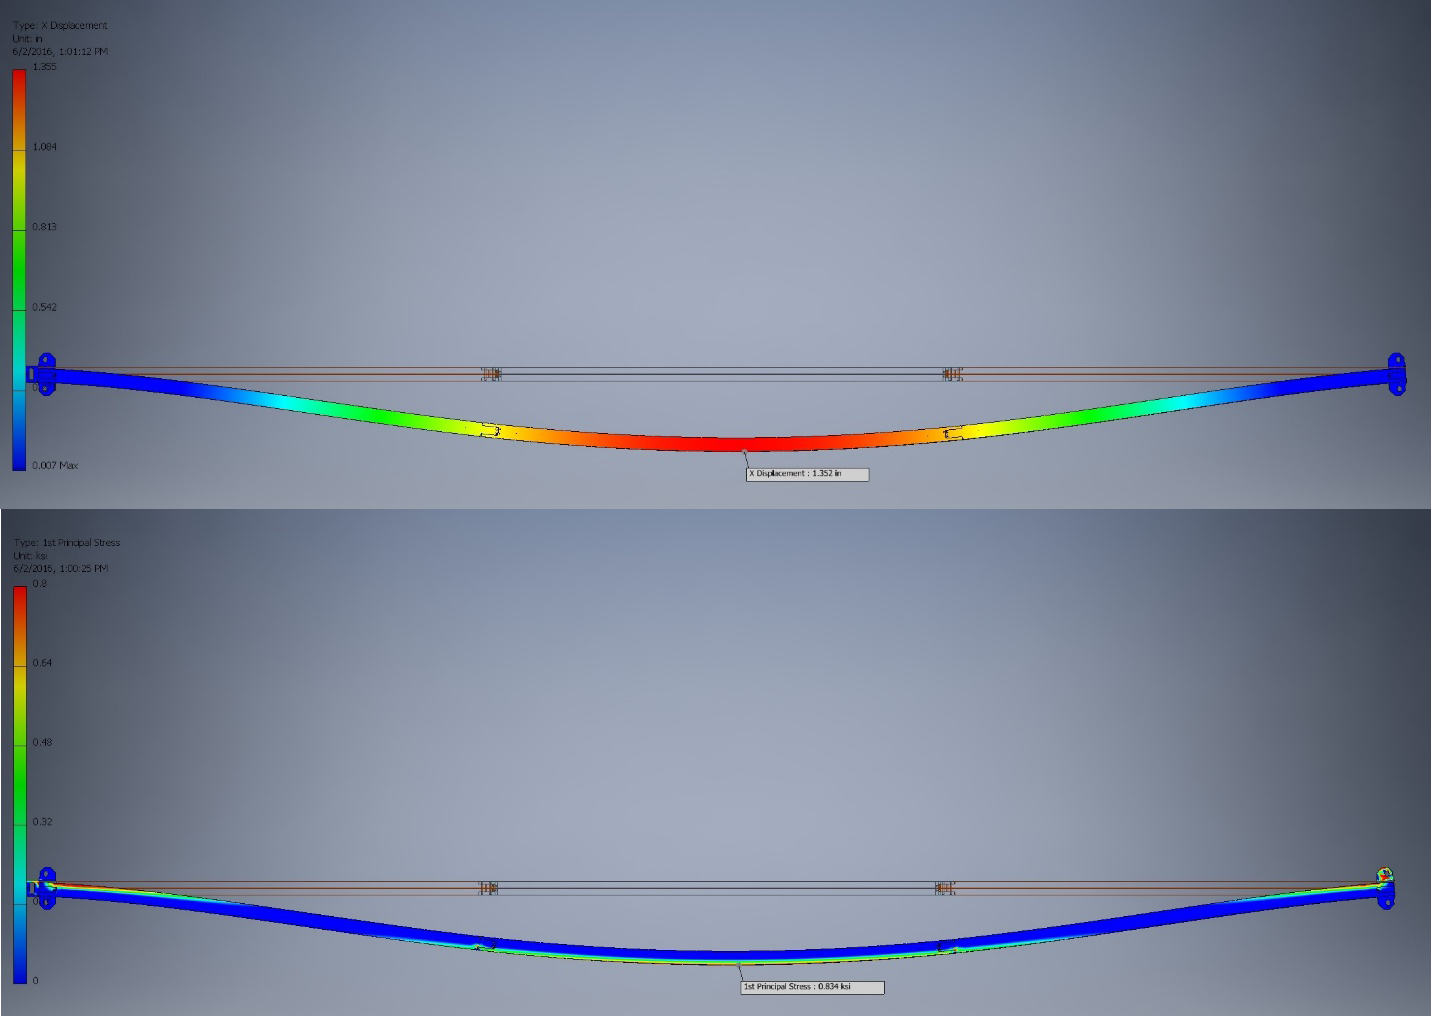
\includegraphics[width=\linewidth]{tpc_cpa_h_load.png}
\end{cdrfigure}


{\it  B. CPA Hanging with all FC Attached in Installation Position}

The current estimate for the FC weight is 440 lbs.  This load is carried by 2 CPAs so each hinge on the CPA will supposed 220 lbs in the installation position.  Figure~\ref{fig:cpa-load1} below shows the deflections and maximum stresses.  The larges deflections are at the bottom cross bar of 0.07'' and the stresses are less than 2,000psi which is far below the ultimate stress of G10.

\begin{cdrfigure}[CPA and 4 FCA load]{cpa-load1}{Stress and deflection of a connected 3 CPA stack suspended on the rail with 4 FC modules} 
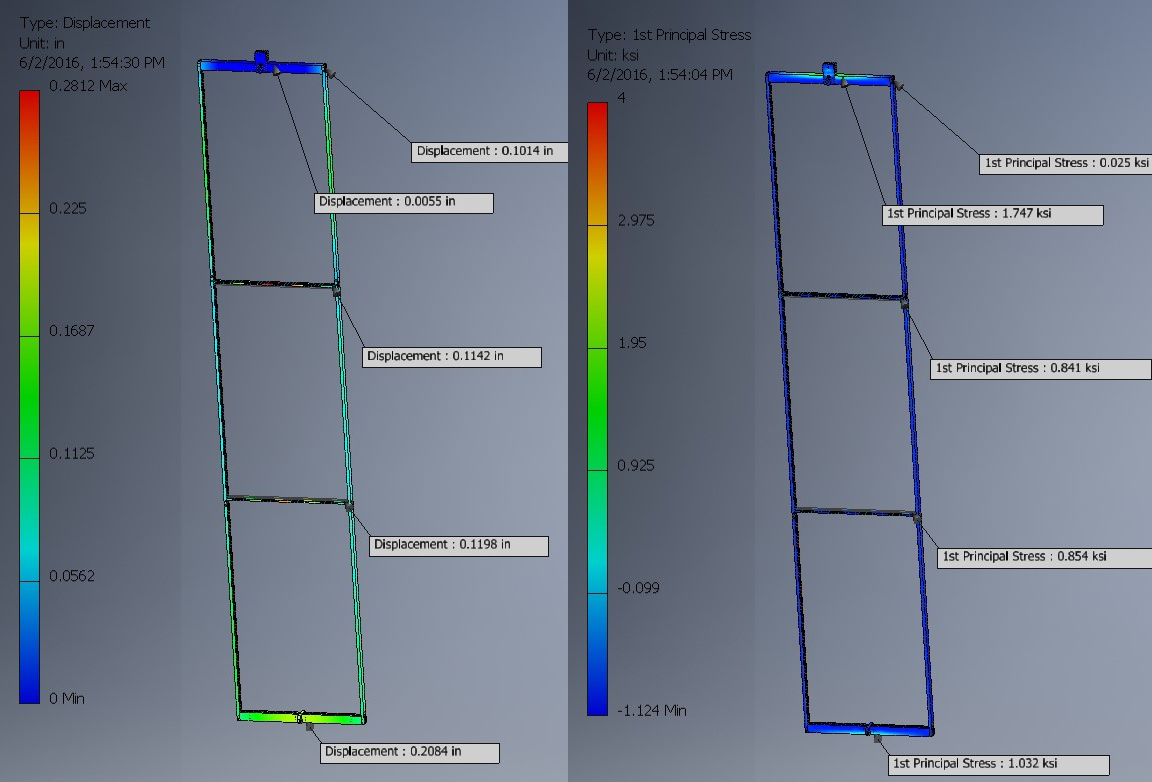
\includegraphics[width=\linewidth]{tpc_cpa_fc_load1.png}
\end{cdrfigure}


{\it  C. CPA Hanging with all FC Attached in Deployed Position With Weight of Workers on FC}

The current estimate for the FC weight is 440 lbs.  This load is carried by 2 CPAs and by the APAs so each hinge on the CPA will supposed 110 lbs in the installation position.  In addition, in the worst case a 200 lbs worker could be standing directly over an I-beam on the FC directly next to a CPA.  The top two hinges on the CPA will have 110 lbs applied.  One of the bottom hinges will have a 110 lbs load also and the second bottom hinge will have 110 lbs of the FC plus the 200 lbs of the worker applied.  The largest deflection is 0.1'' at the bottom cross bar and the stresses are less than 2200psi which is far below the ultimate stress of G10.

\begin{cdrfigure}[CPA load plus 200lb]{cpa-load2}{Stresses and Deflections of CPA with FC Deployed and 200 lb Worker Load} 
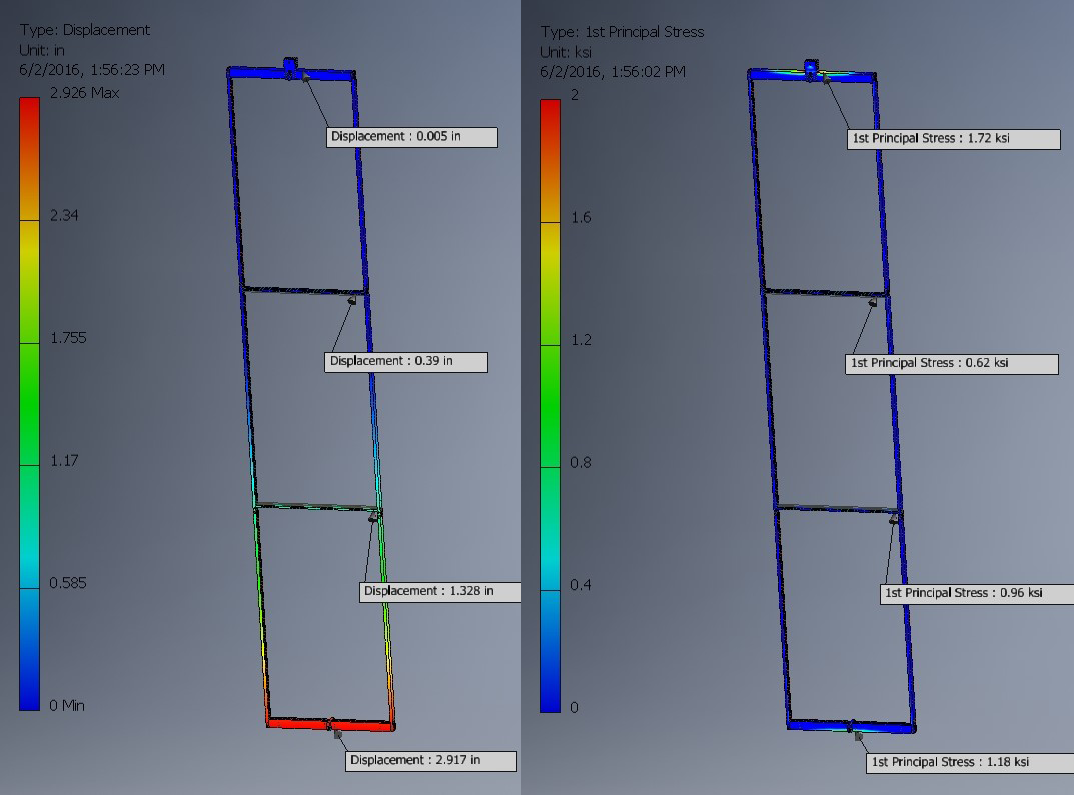
\includegraphics[width=\linewidth]{tpc_cpa_fc_load2.png}
\end{cdrfigure}

{\it D. Connection Stresses}

The weight of the CPA and the bottom FC is transferred through the side bars of the CPA frame.  The connection between the side bars and the top cross bar therefore will experience the highest loads.  A single 1/4'' diameter G10 pin at the connection would have a shear stress of 7740psi which provides a safety factor of greater than 4.  A second pin at each connection would increase the safety factor to 8.  

{\it E. Deformation and Stress Due to Pressure from Circulating Liquid Argon}

Calculations done at FermiLab indicate that a uniform 2Pa pressure during cool down will be applied to the resistive panels.  Calculations show that this will result in 0.090'' deflections of the panel at its center.  The CPA/FC/APA assembly will displace 8.8mm laterally as a result of the next force from this pressure.  

{\it F. Thermal Considerations}

When the CPA modules are cooled their width will shrink by 0.9mm.  The supporting stainless steel beam will shrink by 1.6mm over the width of the CPA.  If the CPA supports are rigidly attached to the supporting stainless steel beam then an interference of 1.6m-.9mm = .7mm will occur.  In order to prevent this interference an initial gap of 0.7mm between CPA’s is required which will insure that the CPAs are in contact after cool down.  

The steel beam between the CPA and APA will cool and shrink by 5.2mm.  The joint between the FC and the CPA must be able to accommodate this shrinkage.


\subsubsection{The HV distribution bus and HV feedthrough receptacle }

Should this be moved to the HV section?

\subsubsection{The mechanical and electrical interconnect features between modules}

There are a stack of 3 modules interconnected vertically to form the 6m height of the SP ProtoDUNE cathode.  The frames of these modules are bolted together using tongue and groove connections at the ends, and the resistive cathode sheets, and the field shaping strips are connected  using a few metallic buttons to ensure redundant electrical contact between vertical modules.

There are 6 columns of the 6m tall CPA modules in SP ProtoDUNE.  Each column is suspended to the CPA rail using a central lifting bar.  Due to the  roof movement between the warm and cold phases of the cryostat, each column is expected to move ~ 2mm relative to its neighbors.  Several pin and slot connections are implemented at the long edges of the CPA columns to ensure the co-planarity of the modules and yet allow small vertical displacement.  The HV bus interconnect the resistive cathode surfaces across the columns to maintain a uniform voltage across the cathode surface.

\subsection{QC Procedures}

